%% abtex2-modelo-projeto-pesquisa.tex, v-1.9.7 laurocesar
%% Copyright 2012-2018 by abnTeX2 group at http://www.abntex.net.br/ 
%%
%% This work may be distributed and/or modified under the
%% conditions of the LaTeX Project Public License, either version 1.3
%% of this license or (at your option) any later version.
%% The latest version of this license is in
%%   http://www.latex-project.org/lppl.txt
%% and version 1.3 or later is part of all distributions of LaTeX
%% version 2005/12/01 or later.
%%
%% This work has the LPPL maintenance status `maintained'.
%% 
%% The Current Maintainer of this work is the abnTeX2 team, led
%% by Lauro César Araujo. Further information are available on 
%% http://www.abntex.net.br/
%%
%% This work consists of the files abntex2-modelo-projeto-pesquisa.tex
%% and abntex2-modelo-references.bib
%%

% ------------------------------------------------------------------------
% ------------------------------------------------------------------------
% abnTeX2: Modelo de Projeto de pesquisa em conformidade com 
% ABNT NBR 15287:2011 Informação e documentação - Projeto de pesquisa -
% Apresentação 
% ------------------------------------------------------------------------ 
% ------------------------------------------------------------------------

\documentclass[
	% -- opções da classe memoir --
	12pt,				% tamanho da fonte
	%openright,			% capítulos começam em pág ímpar (insere página vazia caso preciso)
	%twoside,			% para impressão em recto e verso. Oposto a 
	oneside,
	a4paper,			% tamanho do papel. 
	% -- opções da classe abntex2 --
	%chapter=TITLE,		% títulos de capítulos convertidos em letras maiúsculas
	%section=TITLE,		% títulos de seções convertidos em letras maiúsculas
	%subsection=TITLE,	% títulos de subseções convertidos em letras maiúsculas
	%subsubsection=TITLE,% títulos de subsubseções convertidos em letras maiúsculas
	% -- opções do pacote babel --
	english,			% idioma adicional para hifenização
	french,				% idioma adicional para hifenização
	spanish,			% i      option. Reported}%dioma adicional para hifenização
	brazilian  			% o último idioma é o principal do documento
	]{abntex2}

% ---
% PACOTES
% ---


% ---
% Pacotes fundamentais 
% ---
\usepackage{lmodern}			% Usa a fonte Latin Modern
\usepackage[T1]{fontenc}		% Selecao de codigos de fonte.
\usepackage[utf8]{inputenc}		% Codificacao do documento (conversão automática dos acentos)
\usepackage{indentfirst}		% Indent o primeiro parágrafo de cada seção.
\usepackage{color}				% Controle das cores
\usepackage{graphicx}			% Inclusão de gráficos
\usepackage{microtype} 			% para melhorias de justificação
% ---

\usepackage{csquotes}

% ---
% Math 
% ---
\usepackage{amsfonts, amsmath, amsthm, amssymb}


% ---
% Pacotes adicionais, usados apenas no âmbito do Modelo Canônico do abntex2
% ---
\usepackage{lipsum}				% para geração de dummy text
% ---

% ---
% Pacotes de citações
% ---
%\usepackage[english,hyperpageref]{backref}	 % Paginas com as citações na bibl
%\usepackage[alf]{abntex2cite}	% Citações padrão ABNT
\usepackage[style=abnt]{biblatex}
\addbibresource{biblio.bib}  

% --- 
% CONFIGURAÇÕES DE PACOTES
% --- 

% ---
% % Configurações do pacote backref
% % Usado sem a opção hyperpageref de backref
% \renewcommand{\backrefpagesname}{Cited in page(s):~}
% % Texto padrão antes do número das páginas
% \renewcommand{\backref}{}
% % Define os textos da citação
% \renewcommand*{\backrefalt}[4]{
%     \ifcase #1 %
%         No citation in text.%
%     \or
%         Cited in page #2.%
%     \else
%         Cited #1 times in pages #2.%
%     \fi}%
% % ---

% ---
% Definições de comandos
% ---

\newcommand{\lucas}[1]{\textcolor{red}{#1}}

\theoremstyle{definition}
\newtheorem{definition}{Definition}[section]

% ---
% Informações de dados para CAPA e FOLHA DE ROSTO
% ---
\titulo{Bayesian analysis of respondent-driven surveys with outcome uncertainty}
\autor{Lucas Machado Moschen}
\local{Rio de Janeiro, Brazil}
\data{\today}
\instituicao{%
  Getulio Vargas Foundation -- FGV
  \par
  School of Applied Mathematics
  \par
  Undergraduate Course in Applied Mathematics}
\tipotrabalho{Bachelor Dissertation (Graduation)}
% O preambulo deve conter o tipo do trabalho, o objetivo, 
% o nome da instituição e a área de concentração 
\preambulo{Bachelor dissertation project presented to the School of Applied Mathematics (FGV/EMAp) as a partial requirement for continuing the dissertation work. \\ \\
Advisor: Prof. Luiz Max Carvalho}
% ---

% ---exame2.pdf
% Configurações de aparência do PDF final

% alterando o aspecto da cor azul
\definecolor{blue}{RGB}{41,5,195}

% informações do PDF
\makeatletter
\hypersetup{
     	%pagebackref=true,
		pdftitle={\@title}, 
		pdfauthor={\@author},
    	pdfsubject={\imprimirpreambulo},
	    pdfcreator={LaTeX with abnTeX2},
		pdfkeywords={abnt}{latex}{abntex}{abntex2}{projeto de pesquisa}, 
		colorlinks=true,       		% false: boxed links; true: colored links
    	linkcolor=blue,          	% color of internal links
    	citecolor=blue,        		% color of links to bibliography
    	filecolor=magenta,      		% color of file links
		urlcolor=blue,
		bookmarksdepth=4
}
\makeatother
% --- 

% --- 
% Espaçamentos entre linhas e parágrafos 
% --- 

% O tamanho do parágrafo é dado por:
\setlength{\parindent}{1.3cm}

% Controle do espaçamento entre um parágrafo e outro:
\setlength{\parskip}{0.2cm}  % tente também \onelineskip

% ---
% compila o índice
% ---
\makeindex
% ---

% ----
% Início do documento
% ----
\begin{document}

% Seleciona o idioma do documento (conforme pacotes do babel)
%\selectlanguage{english}
\selectlanguage{english}

% Retira espaço extra obsoleto entre as frases.
\frenchspacing 

% ----------------------------------------------------------
% ELEMENTOS PRÉ-TEXTUAIS
% ----------------------------------------------------------
% \pretextual

% ---
% Capa
% ---
\imprimircapa
% ---

% ---
% Folha de rosto
% ---
\imprimirfolhaderosto
% ---

% ---
% NOTA DA ABNT NBR 15287:2011, p. 4:
%  ``Se exigido pela entidade, apresentar os dados curriculares do autor em
%     folha ou página distinta após a folha de rosto.''
% ---

% ---
% inserir lista de ilustrações
% ---
% \pdfbookmark[0]{\listfigurename}{lof}
% \listoffigures*
% \cleardoublepage
% ---

% ---
% inserir lista de tabelas
% ---
% \pdfbookmark[0]{\listtablename}{lot}
% \listoftables*
% \cleardoublepage
% ---

% ---
% inserir lista de abreviaturas e siglas
% ---
% \begin{siglas}
%   \item[ABNT] Associação Brasileira de Normas Técnicas
%   \item[abnTeX] ABsurdas Normas para TeX
% \end{siglas}
% ---

% ---
% inserir lista de símbolos
% ---
% \begin{simbolos}
%   \item[$ \Gamma $] Letra grega Gama
%   \item[$ \Lambda $] Lambda
%   \item[$ \zeta $] Letra grega minúscula zeta
%   \item[$ \in $] Pertence
% \end{simbolos}
% ---

% ---
% inserir o sumario
% ---
\pdfbookmark[0]{\contentsname}{toc}
\tableofcontents*
\cleardoublepage
% ---

\textual

% ----------------------------------------------------------
% Introdução
% ----------------------------------------------------------
\chapter{Introduction}
%\addcontentsline{toc}{chapter}{Introduction}


This work proposes to study the survey method Respondent-Driven Sampling (RDS), a chain-referral method with the objective of sampling from hard-to-reach populations when necessary to estimate the prevalence of some binary condition from this population. The modeling also accounts for sensibility and sensitivity since the imperfection of the detection tests.  

Hidden or hard-to-reach populations have two main features: no sampling frame
exists, given that their size and boundaries are unknown, and there are
privacy concerns because the subjects are stigmatized or have illegal behavior
\cite{heckathorn1997}. Fear of exposition or prosecution complicates the
enumeration of the populations and the learning about them. Moreover, if the
occurrence frequency of the condition is low, there are high logistic costs
involved. Some examples are heavy drug users, sex workers, homeless people,
and men who have sex with men. 

Researches have been done with the development of some methods to reach these
populations, such as, for example, snowball sampling \cite{goodman1961}, key
important sampling \cite{deaux-callaghan1985}, 
and targeted sampling \cite{watters-biernacki1989}. \citeauthor{heckathorn1997} introduced the Respondent-Driven Sampling (RDS) to
fill some gaps from other methods he depicted in his work. In his proposed
approach, the researchers select a handful of individuals from the target
population and give them coupons to recruit their peers. The individuals
receive a reward for being recruited and for recruiting, which creates a dual
incentive system. After \citeyear{heckathorn1997}, several papers studied this
topic more deeply. 

Following the sampling from the target population, a questionnaire or a
disease test is conducted. This work considers binary outcomes. For
instance, asking about smoking status or testing for HIV infections. However,
the diagnoses are subject to measure error, and regard their accuracy is a
vital step \cite{reitsma2005bivariate}. In particular, we propose the joint
use of sensitivity (the ability to detect the condition) and specificity (the
ability to identify the absence of it).  

Nevertheless, because of our lack of knowledge about nature itself, it is
necessary to model the uncertainty of this process, and Bayesian Statistics is
the indicated area of study. In the Bayesian view, the parameters are random
variables, and the beliefs about them are updated given new data. The idea is
to propagate uncertainty about the outcome through the network of contacts,
which has its probability distribution.

The objective of this work is to analyze the network structure as a stochastic object, along with the sensibility and sensitivity. We also intend to apply this framework efficiently, comparing Monte Carlo algorithms and Laplace approximations.

\section{Respondent-driven sampling}

RDS is commonly used to survey hidden or hard-to-reach populations when
no sampling frame exists \cite{heckathorn1997}. In this approach, the
researchers select some individuals, called {\em seeds} from the target
population, and give them a fixed amount of {\em recruitment coupons} to
recruit their peers. Each recipient of the coupons reclaims it in the study
site, is interviewed, and receives more coupons to continue the recruitment.
This process occurs until it reaches some criteria. The sampling is without
replacement, so the participants cannot be recruited more than once. Moreover,
the respondents inform their {\em network degree}.

The subjects receive a reward for being interviewed and for each recruitment
which establishes a dual system incentive. The {\em primary incentive} is the
{\em individual-sanction-based control}, so there is a reward for
participating. The second one is the {\em group-mediated social control} that
influences the participants seeking to induce others to comply. When social
approval is important, recruitment can be even more efficient and cheaper.
Moreover, the material incentive can be converted into symbolic by the
individuals. 

In a survey, questions about ethnicity, location (not necessarily fixed),
gender, and religion, create possible (finite) states in which each
participant is. By statistical tests, one can verify the association between
the recruiter and recruited responses. \citeauthor{heckathorn1997} models it
as a Markov chain where the states are the possible answers, and the links are
the recruitments. Considering an ergodic chain, an equilibrium mix of recruits
will be attained when the number of waves goes to infinity, and it approaches
the equilibrium at a geometric rate. Therefore, we obtain the distribution of
the states posterior to enough waves. Posterior studies \cite{heckathorn2002}
explained how to access bias and other statistical considerations. 

Besides considering only the states where the individual is located,
\cite{crawford2016} analyses the network structure given by RDS with a
continuous-time model incorporating the recruitment time, the network degree,
and the pattern of coupon use. This configuration enables the treatment of
unobserved links and nodes as missing data. Let $G = (V,E)$ be an undirected
graph representing the hidden population. The {\em recruitment graph} $G_R =
(V_R, E_R)$ represents the recruited individuals and the recruitment edge.
Given that each individual can be sampled only once, it is not possible to
observe the {\em recruitment-induced subgraph}, that is the induced subgraph
generated by $V_R$. Moreover, the {\em coupon matrix} $C$ defined by $C_{ij} =
1$ if the i$^{th}$ subject has at least one coupon before the j$^{th}$
recruitment event, is also observed with the recruitment times. Assuming an
exponential and independent distribution of the times, the likelihood can be
written, and the distribution interpreted as an exponential random graph
model. 

These models allowed several applications in social sciences, epidemiology,
and statistics, including hidden populations size estimation
\cite{crawford2018hidden}, regression \cite{bastos2012binary}, communicable
disease prevalence estimation \cite{albuquerque2009avaliaccao}, among others. 

\section{Prevalence estimation with imperfect tests}

Consider a population of interest and a known condition, such as, for example,
a disease or a binary behavior. It is important to understand the proportion
of individuals in this population exposed at time $t$, called {\em
prevalence}. Suppose a diagnostic test is done to measure the presence or the
absence of this condition in the individuals. Mathematically, let $\theta \in
(0,1)$ be the prevalence (parameter of interest) of the condition and $Y_i$ be an indicator function of the presence of the condition in the i$^{th}$ individual.
Assuming for simplicity that all tests are performed at time $t$, and the
sample is $\{y_1, ..., y_n\}$, the maximum likelihood estimator is the
apparent prevalence: 
\begin{equation}
    \label{eq:naive-estimator}
    \hat{\theta} = \frac{1}{n}\sum_{i=1}^n y_i.
\end{equation}
However, this estimator has two problems in this context: it assumes a perfect
diagnostic test, which is often incorrect, and the samples in RDS are not
independent by definition (network structure). 

The first problem in \eqref{eq:naive-estimator} was tackled several times in
the literature, such as \cite{mcinturff2004modelling}. The diagnose accuracy
can be measured in many ways and the most considered is the joint analysis of
the {\em sensitivity} ($\gamma_s$) and the {\em specificity}
($\gamma_e$). 

\begin{definition}[Specificity]
    It is the probability of a negative test conditioned on the absence of the
    disease (true negative).
\end{definition}

\begin{definition}[Sensitivity]
    It is the probability of a positive test conditioned on the presence of
    the disease (true positive). 
\end{definition}

Let $p$ be the probability of a positive test. Then, by Law of Total
Probability: 
\begin{equation}
    p = \theta\gamma_s + (1-\theta)(1-\gamma_e).    
\end{equation}

Establishing a link function in $(\theta, \gamma_s, \gamma_e)$, it is possible
to use linear regression and prior distributions to the regressors
$\boldsymbol{\beta}$ to estimate $\theta$ conditioned on data. One important
additional problem is to consider the correlation between $\gamma_s$ and $\gamma_e$. 


The second problem was a study object in \cite{heckathorn1997,heckathorn2002} where the estimator was proposed
based largely on Markov chain theory and social network theory.
\cite{volz2008probability} improved it with the RDS II estimator considering
the network degree
\begin{equation}
    \hat{\theta}^{RDS II} = \frac{\sum_{i=1}^n y_i \delta_i^{-1}}{\sum_{i=1}^n \delta_i^{-1}},
\end{equation}
such that $\delta_i$ is the i$^{th}$ individual's degree. However, this is an
area of research in progress. 

\section{Bayesian statistics}

There are two more common interpretations of probability and statistics:
frequentist and Bayesian. While the frequentists define
probability as the limit of a frequency in a large number of trials, the
Bayesians represent an individual's degree of belief in a statement that is
updated given new information. This philosophy allows assigning probabilities
to any event, even if a random process is not defined \cite{statisticat2016laplacesdemon}. 

In 1761, Reverent Thomas Bayes wrote for the first time the Bayes' formula
relating the probability of a parameter after observing the data with the
evidence (written through a likelihood function) and previous information
about the parameter. Pierre Simon Laplace rediscovered this formula in 1773
\cite{Robert2007}, and this theory became more common in the 19th century.
After some criticisms, a modern treatment considering Kolmogorov's axiomatization of the theory of probabilities started after Jeffreys in 1939.
The recent development of new computational tools brought these ideas again.

Bayesian inference is composed by the following: 

\begin{itemize}
    \item A distribution for the parameters $\theta$ that quantifies the
    uncertainty about $\theta$ before data;
    \item A distribution of the data generation process given the parameter,
    such that, when it is seen as function of the parameter, is called
    likelihood function;
    \item When considering decision theory, a loss function indicating a
    measure of error;
    \item Posterior distribution of the parameter conditioned on the data. All
    inferences are based on this probability distribution.
\end{itemize} 

\chapter{Justification}

There are two justifications for the importance of this work. First, hidden
populations are often omitted from national representative surveys since they
do not have fixed addresses and cannot be reached, or they fear prosecution
after showing themselves. However, the individuals can
have a greater risk of drug abuse or having sexually transmitted infections.
This combination creates an environment of aid absence from the government to
these people. The second reason is mathematical. This topic has lots of gaps
in Statistics that deserve attention. The correct sampling probabilities for
the recruited members under RDS are hard to obtain since not all links and
nodes are observed, constituting missing data \cite{crawford2016}. In this fertile area,
regression approaches to prevalence estimation taking the network structure
can be built \cite{bastos2012binary} and are still in development.

\chapter{Objectives}

\section{Main}

The objective of this work is to analyze the network structure of RDS as a
stochastic object, along with the sensibility and sensitivity. We also intend
to apply this framework efficiently, comparing Monte Carlo algorithms and
Laplace approximations.



\section{Specifics}

\begin{alineas}
    \item Bibliography review including possible mathematical formulations of
    RDS, logistic regression when the outcome has uncertainty (imperfect
    tests) and applications in hidden or hard-to-reach populations; 

    \item Problem description in mathematical terms considering the
    uncertainty in the network (missing data in the RDS) and the
    diagnose. Uncertainty propagation; 

    \item Bayesian methods and prior calibration. Prior predictive checking on
    the positive test probability when there are weak priors of the
    regression parameters; 

    \item Efficient implementation using statistical packages, as {\em
    rstanarm} \cite{rstanarm} and {\em INLA} \cite{rue2009approximate}. Comparison between MCMC and Laplace
    approximation; 

    \item Analysis of RDS epidemiological studies.
\end{alineas}

\chapter{Methodology}

{\em Document Research:}

The theoretical foundation will be through papers in the topics indicated in
the introduction, RDS, bayesian statistics, and prevalence estimation through
regression. 

{\em Technical resources:}

All the necessary programming will be done in the programming languages
\textit{Python} and \textit{R}, given the simple connection to data processing
and
statistics. 

{\em Formal studies}

In order to help the learning about the foundations, two subjects from the
PhD in Mathematical Modelling at EMAp will be taken: Bayesian Statistics and
Network Science. The first one ended in June, while the second will be
finished on September.  

\chapter{Preliminary results}
\label{sec:preliminary}

\begin{alineas}
    \item Descrição do problema em termos matemáticos e revisão bibliográfica:
    material sobre RDS (formalização matemática em forma de cadeia ou processo
    de ramificação), regressão logística em que a resposta tem incerteza e
    aplicações em usuários de drogas, infecções transmissíveis, entre outros. 
    \item Incerteza sobre especificidade e sensitividade do teste e como
    propagar a classificação errada na rede. Comparação de prioris e, por isso, estudo de
    métodos Bayesianos. Justificar utilização desses métodos com argumento da
    incerteza. 
    \item Estudo do MCMC e Aproximação de Laplace, comparação dos algoritmos
    em alguns artigos e, quem sabe, codificação em Python e R. 
    \item Implementação de inferência eficiente em INLA, com possibilidades
    abertas em Python (talvez Julia?)
\end{alineas}

\chapter{Schedule}

A tentative schedule is depicted in Figure \ref{fig:schedule}. 

\begin{figure}[!ht]
    \centering
    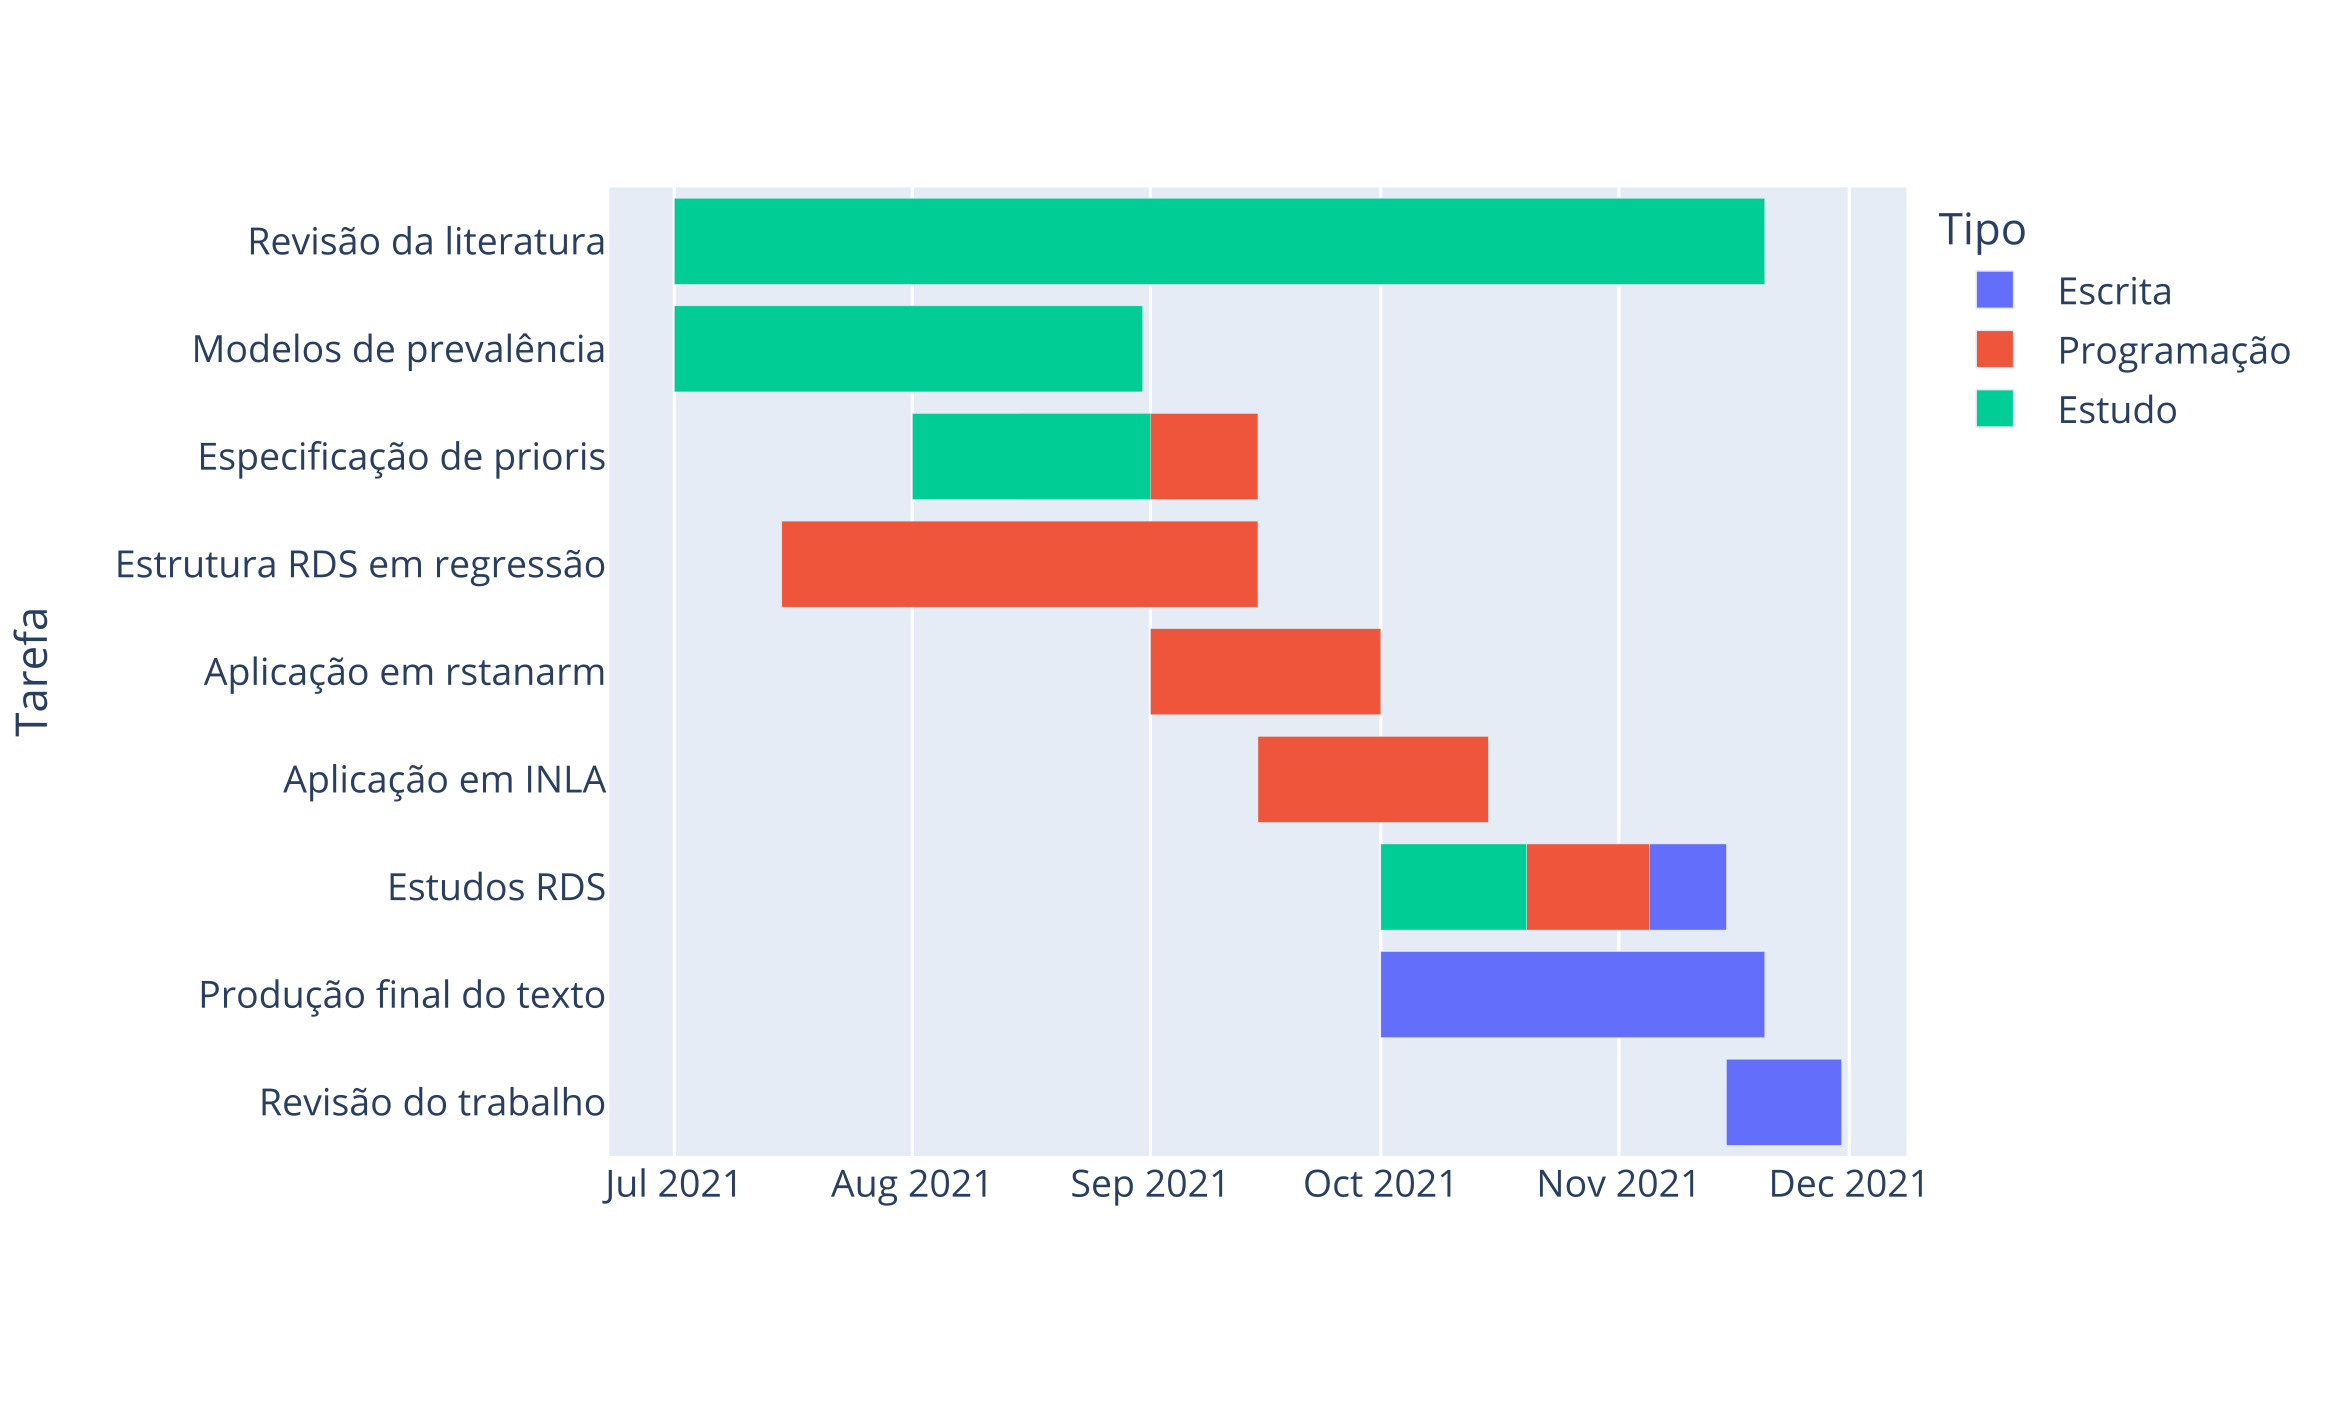
\includegraphics[width = \textwidth]{../../images/gantt-chart-schedule.png}
    \caption{Tentative schedule for the project during the second semester of 2021.}
    \label{fig:schedule}
  \end{figure}

\phantompart

% ---
% Conclusão
% ---
% \chapter*[Considerações finais]{Final considerations}
% \addcontentsline{toc}{chapter}{Final considerations}

\postextual

% ----------------------------------------------------------
% Referências bibliográficas
% ----------------------------------------------------------

%\bibliography{biblio}
\printbibliography

% ----------------------------------------------------------
% Glossário
% ----------------------------------------------------------

%\glossary

% ----------------------------------------------------------
% Apêndices
% ----------------------------------------------------------

\begin{apendicesenv}

% \partapendices

\end{apendicesenv}
% ---


% ----------------------------------------------------------
% Anexos
% ----------------------------------------------------------

\begin{anexosenv}

% \part anexos

\end{anexosenv}

%------------------------------------------------------------
% ÍNDICE REMISSIVO
%------------------------------------------------------------

\phantompart

\printindex


\end{document}
